% Use-case figure: separately converted files joined by shared identifiers, the
% policy layer, and what each requester receives (vcf-rdfizer-testing
% experiment 17; numbers from its comparison.json files, 2026-09-28 to 09-30).
% Standalone TikZ source; build with: pdflatex fig-usecase.tex -> fig-usecase.pdf
% Drawn at the journal text width (372pt, about 13.1 cm) so it is included unscaled.
\documentclass[border=2pt]{standalone}
\usepackage[T1]{fontenc}
\usepackage{helvet}
\renewcommand{\familydefault}{\sfdefault}
\usepackage{tikz}
\usetikzlibrary{arrows.meta,positioning,calc}

% The policy figure's palette: data, files, identifiers (as selections), policy.
\definecolor{crec}{HTML}{DDEFEF}  \definecolor{crecd}{HTML}{1F7F83}
\definecolor{cfile}{HTML}{F6E3B4} \definecolor{cfiled}{HTML}{C9A227}
\definecolor{csel}{HTML}{F2F2F0}  \definecolor{cseld}{HTML}{6E6D68}
\definecolor{cpol}{HTML}{E8E4F7}  \definecolor{cpold}{HTML}{4A3AA7}

\newcommand{\head}{\bfseries}

\begin{document}
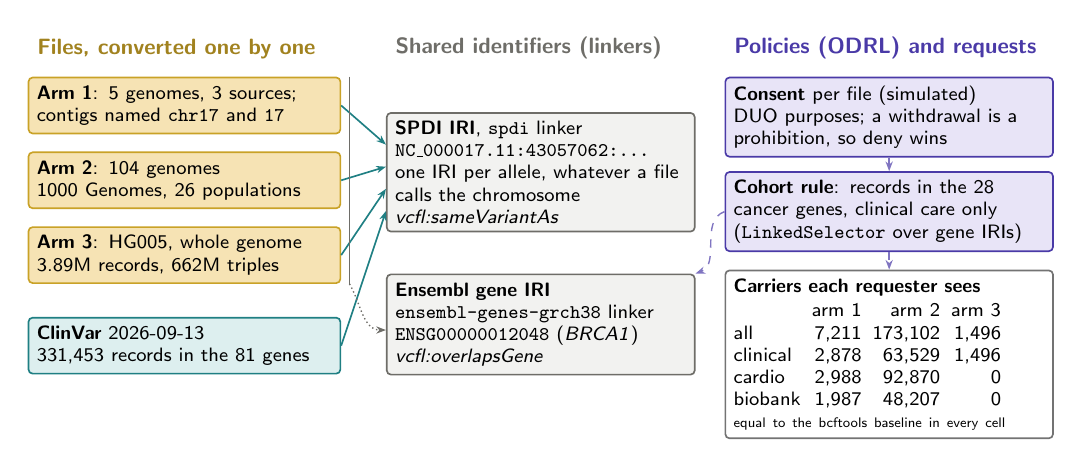
\begin{tikzpicture}[
  font=\scriptsize,
  box/.style={draw, rounded corners=1.5pt, line width=0.6pt, align=left, inner sep=3pt,
              text width=#1, anchor=north west},
  lane/.style={font=\footnotesize\bfseries\itshape, anchor=south west},
  link/.style={-{Stealth[length=3.5pt]}, line width=0.6pt, draw=crecd},
  gene/.style={-{Stealth[length=3.5pt]}, line width=0.5pt, draw=cseld, densely dotted},
  target/.style={-{Stealth[length=3.5pt]}, line width=0.5pt, draw=cpold!70, dashed},
  p/.style={font=\tiny\itshape, fill=white, inner sep=0.8pt},
]

% ------------------------------------------------------------ lanes
\node[lane, text=cfiled!80!black] at (0,0.1) {Files, converted one by one};
\node[lane, text=cseld] at (4.55,0.1) {Shared identifiers (linkers)};
\node[lane, text=cpold] at (8.85,0.1) {Policies (ODRL) and requests};

% ------------------------------------------------------------ files
\node[box=3.75cm, fill=cfile, draw=cfiled] (arm1) at (0,0) {%
  {\head Arm 1}: 5 genomes, 3 sources;\\ contigs named \texttt{chr17} and \texttt{17}};
\node[box=3.75cm, fill=cfile, draw=cfiled] (arm2) at (0,-0.95) {%
  {\head Arm 2}: 104 genomes\\ 1000 Genomes, 26 populations};
\node[box=3.75cm, fill=cfile, draw=cfiled] (arm3) at (0,-1.9) {%
  {\head Arm 3}: HG005, whole genome\\ 3.89M records, 662M triples};
\node[box=3.75cm, fill=crec, draw=crecd] (clinvar) at (0,-3.05) {%
  {\head ClinVar} 2026-09-13\\ 331{,}453 records in the 81 genes};

% ------------------------------------------------------------ identifiers
\node[box=3.7cm, fill=csel, draw=cseld] (spdi) at (4.55,-0.45) {%
  {\head SPDI IRI}, \texttt{spdi} linker\\
  \texttt{NC\_000017.11:43057062:\dots}\\
  one IRI per allele, whatever a file\\ calls the chromosome\\
  {\itshape vcfl:sameVariantAs}};
\node[box=3.7cm, fill=csel, draw=cseld] (gene) at (4.55,-2.5) {%
  {\head Ensembl gene IRI}\\ \texttt{ensembl-genes-grch38} linker\\
  \texttt{ENSG00000012048} (\textit{BRCA1})\\
  {\itshape vcfl:overlapsGene}};

\draw[link] (arm1.east) -- ([yshift=10pt]spdi.west);
\draw[link] (arm2.east) -- ([yshift=2pt]spdi.west);
\draw[link] (arm3.east) -- ([yshift=-6pt]spdi.west);
\draw[link] (clinvar.east) -- ([yshift=-14pt]spdi.west);
% Every genome's calls, not ClinVar's, are also linked to the genes they overlap.
\draw[line width=0.5pt, draw=cseld] ([xshift=3pt]arm1.north east) -- ([xshift=3pt]arm3.south east)
  coordinate[pos=1] (bracket);
\draw[gene] (bracket) to[out=-60, in=180] ([yshift=-2pt]gene.west);

% ------------------------------------------------------------ policies
\node[box=3.95cm, fill=cpol, draw=cpold] (consent) at (8.85,0) {%
  {\head Consent} per file (simulated)\\ DUO purposes; a withdrawal is a\\ prohibition, so deny wins};
\node[box=3.95cm, fill=cpol, draw=cpold] (rule) at (8.85,-1.2) {%
  {\head Cohort rule}: records in the 28\\ cancer genes, clinical care only\\
  (\texttt{LinkedSelector} over gene IRIs)};
\draw[target] (rule.west) to[out=200, in=20] (gene.north east);

% ------------------------------------------------------------ answers
\node[box=3.95cm, draw=black!55, fill=white] (answer) at (8.85,-2.45) {%
  {\head Carriers each requester sees}\\[1pt]
  \setlength{\tabcolsep}{2pt}%
  \begin{tabular}{@{}lrrr@{}}
           & arm 1 & arm 2 & arm 3 \\
  all      & 7{,}211 & 173{,}102 & 1{,}496 \\
  clinical & 2{,}878 & 63{,}529 & 1{,}496 \\
  cardio   & 2{,}988 & 92{,}870 & 0 \\
  biobank  & 1{,}987 & 48{,}207 & 0 \\
  \end{tabular}\\[1pt]
  {\tiny equal to the bcftools baseline in every cell}};
\draw[target] (consent.south) -- (rule.north);
\draw[target] (rule.south) -- (answer.north);
\end{tikzpicture}
\end{document}
